\documentclass[10pt, handout]{beamer}

%\usepackage[backend=bibtex,firstinits=true,style=verbose-inote,citestyle=authortitle]{biblatex}
\usepackage{bm}
\usepackage{graphicx}
\usepackage{subcaption}
\usepackage{amsmath}
\usepackage{amsfonts}
\usepackage{makecell}
\usepackage{filecontents}
\usepackage{biblatex}
\newcommand{\expect}[2][]{
\ifthenelse{\equal{#1}{}}{
\mathbb{E}\left[#2\right]
}{
\underset{#1}{\mathbb{E}}\left[#2\right]
}}

\newcommand{\cov}[2][]{
\ifthenelse{\equal{#1}{}}{
\text{Cov}\left[#2\right]
}{
\underset{#1}{\text{Cov}}\left[#2\right]
}}


\newcommand{\var}[2][]{
\ifthenelse{\equal{#1}{}}{
\text{Var}[#2]
}{
\underset{#1}{\text{Var}}[#2]
}}

\newcommand{\loss}[2][]{
\ifthenelse{\equal{#1}{}}{
\mathcal{L}(#2)
}{
\mathcal{L}_{#1}(#2)
}}

\newcommand{\kl}[2]{
\text{D}_\text{KL}[#1 \parallel #2]
}

\newcommand{\R}{\mathbb{R}}
%\newcommand{\Prob}{\mathbb{P}}

\newcommand{\1}[1]{\mathds{1}\{#1\}}


%\usecolortheme{dolphin}
\setbeamertemplate{navigation symbols}{}
\setbeamertemplate{section in toc}{\inserttocsectionnumber.~\inserttocsection}

\addbibresource{references.bib}


\title{Meta Generation}
%\subtitle{}
\author{Ivan Skorokhodov}
%\date{}
%\logo{
\includegraphics[height=1cm]{images/ipavlov-logo.png}}

\newcommand{\citepaper}[1]{\citetitle{#1} by \citeauthor{#1}}

%\graphicspath{{./images}}

%\usetheme{lucid}
\begin{document}

\begin{frame}
    \titlepage
\end{frame}


\begin{frame}{Implicit Neural Representations}
\begin{itemize}
    \item\pause INR is a neural network $f_\varphi(x,y)$ which takes coordinates $(x,y)$ and produces a pixel value:
    \begin{figure}
        \centering
        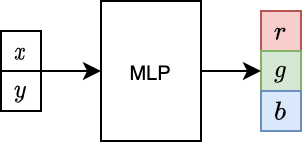
\includegraphics[width=0.3\textwidth]{images/inr}
    \end{figure}
    \item\pause We can generate the whole image by computing the value of $f_\varphi(x,y)$ at each coordinate
    \item\pause I.e. we have \textit{1 image} = \textit{1 INR}
\end{itemize}
\end{frame}


\begin{frame}{Benefits of INRs}
    \begin{itemize}
        \item\pause They carry more ``complete'' information about a signal:
        \begin{itemize}
            \item Usual 2D arrays of pixels are discretized version of a signal
            \item INRs are continuous and carry information ``between'' the pixels
            \item This allows one to have ``superresolution out-of-the-box''
        \end{itemize}
        \item\pause They are popular in 3D deep learning since they are cheaper to generate and operate with than 3D objects
        \begin{itemize}
            \item\pause For 2D images the situation is not currently clear
        \end{itemize}
    \end{itemize}
\end{frame}


\begin{frame}{Problems with INRs}
\begin{itemize}
    \item\pause INRs are not that small:
    \begin{itemize}
        \item\pause SIREN/FFN use $\approx 256\times 5$ MLPs with 3000 epochs
        \item\pause But fitting low-frequency images is much easier\footnote{a note to myself: show face/knot examples here}
    \end{itemize}
    \item\pause It requires to train an INR on an image to obtain the INR and each training procedure (currently) takes a lot of time (up to 10 minutes).
    \item\pause Community does not have a good understanding of how to work with them
\end{itemize}
\end{frame}


\begin{frame}{Transposed convolutions are problematic}
\begin{itemize}
    \item\pause They lack the biological plausibility of normal convolutions
    \item\pause They produce artefacts (like checkerboard patterns)
    \item\pause You have to change architecture for each output size
    \begin{itemize}
        \item\pause This can be solved by interpolation procedures to some extent, but for tasks like segmentation this would lead to coarse predictions
    \end{itemize}
    \item\pause They struggle to capture scene geometry:
    \begin{itemize}
        \item\pause For example, it's hard to draw long straight lines (so generated walls ``wobble'', circles are curved, etc)
        \item\pause CoordConv paper showed that it cannot learn to classify a pixel given its coordinates
    \end{itemize}
\end{itemize}
\end{frame}



\begin{frame}{INR-GAN}
\begin{itemize}
    \item\pause Main idea: train a generator to produce INRs
    \begin{figure}
        \centering
        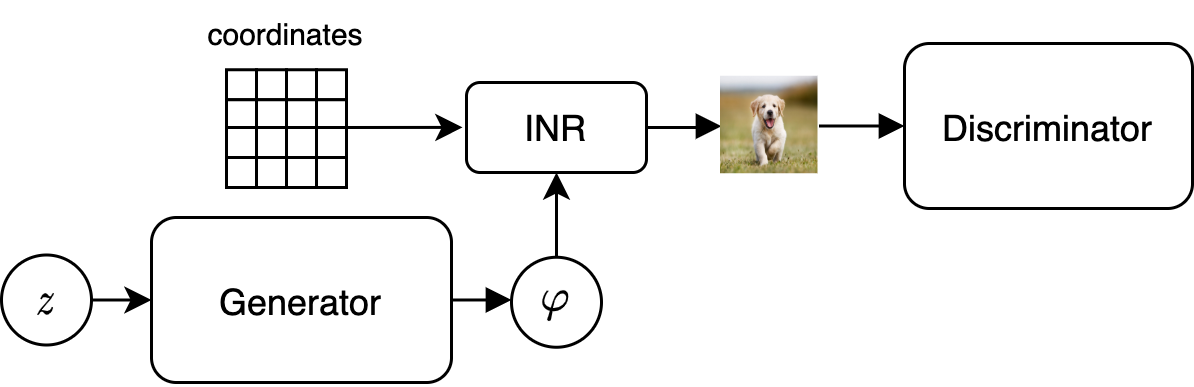
\includegraphics[width=0.9\textwidth]{images/inr-gan}
    \end{figure}
    \item\pause Discriminator can operate:
    \begin{itemize}
        \item\pause on top of images
        \item\pause on top of INRs (but this would require converting the whole dataset into INRs)
    \end{itemize}
\end{itemize}
\end{frame}


\begin{frame}{Pros and cons}
Pros
\begin{itemize}
    \item\pause Unified Generator architecture for any domain (images/3D-images/video/audio) since all of them are ``representable'' by INRs
    \item\pause Easier super resolution
    \item\pause Easier progressive growing in Generator
    \item\pause It should be easer to capture the geometry\footnote{a note to myself: show CoordConv here}
    \item\pause Better biological plausibility
\end{itemize}

Cons
\begin{itemize}
    \item\pause I have no idea how hard it is to accomplish
    \item\pause It can be the case that everyone has the idea of INR-GAN like models (after SIREN and FFNs)
    \item\pause StyleGAN has a ton of tricks and will be extremely hard to beat
\end{itemize}
\end{frame}


\begin{frame}{Meta Generation}
    \begin{itemize}
        \item\pause \textit{A more general idea}:
        \begin{itemize}
            \item\pause let Decoder take a coordinate + smth (noise? embedding?) and output a pixel value
            \item\pause let Generator take smth (noise? embedding?) and produce smth (weights? embedding?) to control\footnote{To ``neuromodulate'' it --- this is a bialogically plausible motivation of hypernetworks} Decoder (in the extreme situation, Generator outputs all the Decoder's weights)
        \end{itemize}
        \item\pause This is pretty similar to StyleGAN
        \item\pause Ideally, we would like to produce a decoder that can generate a single object (like face identity) in different conditions (lightning, zoom, position, etc)
%        \item\pause This is a very general idea and can be achieved with some modifications of INRs (i.e. sharing weights between images, conditioning on something, etc).
    \end{itemize}
\end{frame}



%\begin{frame}{Resemblance to StyleGAN}
%StyleGAN can be seen as INR-GAN:
%\begin{itemize}
%    \item\pause Its decoder is an INR, its
%    \item\pause It has shared weights between different 
%\end{itemize}
%\end{frame}


\begin{frame}{Questions}
    \begin{itemize}
        \item How to make INRs cheaper?
        \item How can we share weights in different decoders (to make INRs cheaper)?
        \item How can we control Decoder with Generator?
    \end{itemize}
\end{frame}

\end{document}
